\section{Compresi�n PPMC}

Como en los dem�s compresores implementados, se realiz� una separaci�n entre el compresor y el descompresor. 
Las clases y las interfaces son relativamente simples. Existe sin embargo funcionalidad exactamente igual en ambos, 
con lo cual algunas cosas se generalizaron.

\begin{figure}[!htp]
\centering
\makebox[\textwidth]{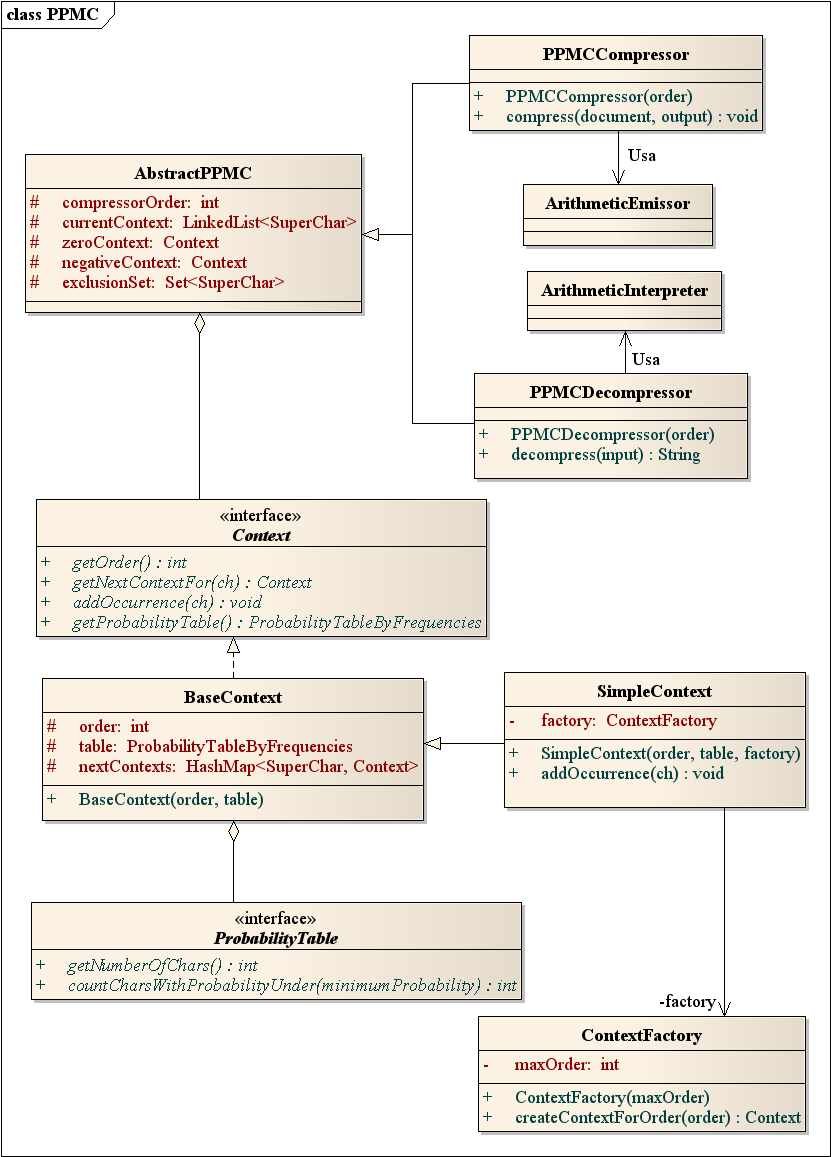
\includegraphics[scale=0.5,natwidth=20pt,natheight=10pt,width=0.70\textwidth]{img/PPMC.png}}
	\caption{Diagrama de clases general de la arquitectura}
\end{figure}

\subsection{Compresor PPMC}
Se crea un compresor indicando el orden a utilizar (hasta 4) y opcionalmente puede recibir un PrintStream en el que ir�
logueando informaci�n de debugging que puede ser �til (que se est� emitiendo en cada caso, y como quedan los contextos).
Para comprimir un documento, se le debe pasar al compresor un \textit{Document} y un \textit{OutputBuffer} en el que ir�
guardando el resultado de la descompresi�n. 
Al igual que en el LZP, el buffer es utilizado para crear un compresor aritm�tico. El aritmetico va comprimiendo los
caracteres que el PPMC le vaya pasando, junto con la tabla de probabilidad del contexto adecuado (de esto �ltimo 
obviamente se encarga el Compresor PPMC). El aritm�tico env�a los bits correspondientes a la compresi�n al buffer.

\subsection{Descompresor PPMC}
El descompresor se crea de la una manera identica al compresor, es decir, se le puede pasar el orden a utilizar y un
PrintStream.
Para la descompresi�n se le debe pasar un \textit{InputBuffer} que contenga el mensaje a descomprimir. Se utiliza un
Aritm�tico que interpreta los bits segun las tablas de probabilidad que le pase el descompresor PPMC. El aritm�tico lee
los bits desde el InputBuffer recibido.
Despu�s de realizar la descompresi�n de todos los caracteres (y encontrar un \textit{End-Of-File}) se devuelve un String
que representa el mensaje original.

\subsection{Contextos}
Tanto el compresor como el descompresor utilizan una estructura id�ntica de contextos para mantener un estado coherente.
La forma de implementar esto, como se mostr� en la arquitectura propuesta, fue la de crear una estructura de contextos 
encadenados.
El compresor/descompresor PPMC tienen a su alcance los contextos de orden 0 y de orden -1. A partir del orden 0, se 
puede encontrar cualquier contexto utilizando una List que indique el contexto buscado (Por ejemplo puede contener 
[A,B,C] y se buscara el contexto correspondiente a "ABC").
Cada contexto tiene una tabla de probabilidad que registra las ocurrencias de caracteres para ese contexto. Se pueden
agregar ocurrencias de caracteres al contexto, que repercutiran en agregar ocurrencias de caracteres en la tabla.

\subsubsection{Tipos de Contextos}
Se crearon 2 tipos de contextos, un contexto base con una implementaci�n b�sica y un contexto que permite encadenar m�s
contextos. Si bien no difieren demasiado entre s�, tienen la diferencia importante de poder o no encadenar contextos.
El contexto base es utilizado en el orden -1 y en el ultimo orden posible. El otro tipo de contexto es utilizado en los
ordenes 0 a n-1.
Este �ltimo permite que al agregar una ocurrencia de un caracter al contexto, si el caracter no exist�a previamente en
dicho contexto, se crea un nuevo contexto del tipo adecuado, y se linkea contra este contexto.

\subsection{Algoritmo de Compresi�n y Descompresi�n}
El algoritmo utilizado para la compresi�n y la descompresi�n es bastante similar en esencia. Se tiene una representaci�n
en caracteres del contexto actual y se utiliza para saber que contextos ser� necesario acceder. 
Se parte del contexto de orden 0 y se recorren los contextos recursivamente. Generalmente se llega al �ltimo contexto 
(de orden n) y se realiza el proceso de emisi�n recorriendo los contextos, finalizada est� parte se hacen 
actualizaciones en las tablas si es necesario. 
El contexto de orden -1 es generalmente tratado de manera distinta, ya que aqu� no hay que agregar ocurrencias de 
caracteres sino eliminar caracteres una vez que fueron emitidos.

\subsubsection{Exclusi�n completa}
Para aplicar exclusi�n completa simplemente se crea un \textit{Set} (\textit{HashSet}) al iniciar la descompresi�n y se
van agregando los caracteres que necesitan excluirse. De esta manera cada vez que se va a emitir algo, se aplica antes
a la tabla de probabilidades este set de exclusi�n.

\subsection{Serializer}

Para integrar el compresor con nuestra arquitectura, fue necesario crear un \textit{PPMCSerializer} que utiliza el 
compresor y descompresor PPMC para hidratar y deshidratar Documentos.
